\chapter{A Method for Application}
\textit{``I hate portals''} \\
\rightline{Geralt of Rivia} \\
\rightline{The Withcer 3: Wild Hunt \cite{witcher}}

\section{A Delegation of Effort}
When having used the framework for analysis, it is clear that use in a design context would not be constructive, since the complexity necessitates a high degree of absorption and, most importantly, loads of time. Therefore, for the creation of a practical method, I decided to delegate the effort into two parts taking place during well-known processes in game development: playtesting and ideation. To test the effectiveness of the proposed method, I gathered a group of experienced game developers who, importantly, have not undertaken the same education specialisation as me, which assisted the developing of a universal method, and avoided the method specifying into a narrow school of thought. Another benefit of the test group was that they had previously worked on games together which limited the amount of noise arising from not knowing each others' approaches to game development, and assuring a solid baseline for comparison to previous development situations. The testing was separated into three phases corresponding to the two processes of playtesting and ideation. The first phase consisted of a playtesting situation with a prototype video game made by me specifically for the test following the ideas presented in \citeA{prototype}. I, then, acted as the interviewer and each group member acted in turn as the playtester. The second phase consisted of the group being presented with a drawn model on a whiteboard representing the simplified framework and the data I had gathered from the playtest. The third and last phase consisted of a semi-structured focus group interview \cite{cresswell} where the participants had a chance to discuss their impressions. The method for gathering qualitative data was chosen to be a focus group. This method was chosen because it is effective in gathering data from a group of respondents \cite{cresswell}, and since the target group for the method is a game development team, this was deemed suitable.

The main goal of the prototype video game was for it to be used as a tool for evaluating the proposed method, so the most important aspect was identified as the prototype aspiring to be as original as possible. The intent of this was to disconnect previous experiences the test participants might have had if the prototype had been similar to a game they had played previously, thereby optimistically limiting unknown variables in the evaluation. Realising that creating something original is a perilous task, an emphasis was simply put on implementing as few as possible conventional game mechanics such as using the W, A, S and D key for movement. Consequently, movement in the prototype is controlled by a mouse-wheel with the playable figure also resembling this wheel (see figure \ref{prototype}). The prototype consists of three minor challenges to ground the player in the control scheme and one integral kinaesthetic challenge as the focus of the test. This kinaesthetic challenge can be seen in figure \ref{prototype}. It consists of two doorways, one from which the player enters and the other through which the player needs to exit. Between the two doorways is a lowered area creating a gap between the two which makes travelling from one doorway directly to the other impossible since the playable figure cannot inherently move vertically. Leaning on the pathway leading into the room is a large barrel oriented horizontally which is suspended off the lower ground by a round beam going through the barrel's centre. The beam is held up by its extremities lying in two grooves in the walls perpendicular to the doorways. Lastly, the room is sloping toward the entrance making the entrance level slightly lower than the exit. The intended strategy to get to the other side is then to position the playable figure, a wheel, on top of the barrel and then use the weight of the wheel to rotate the barrel, which rotates the beam that progresses everything forward towards the exit where the player can climb off the barrel and exit.

\begin{wrapfigure}{i}{0.6\textwidth}
  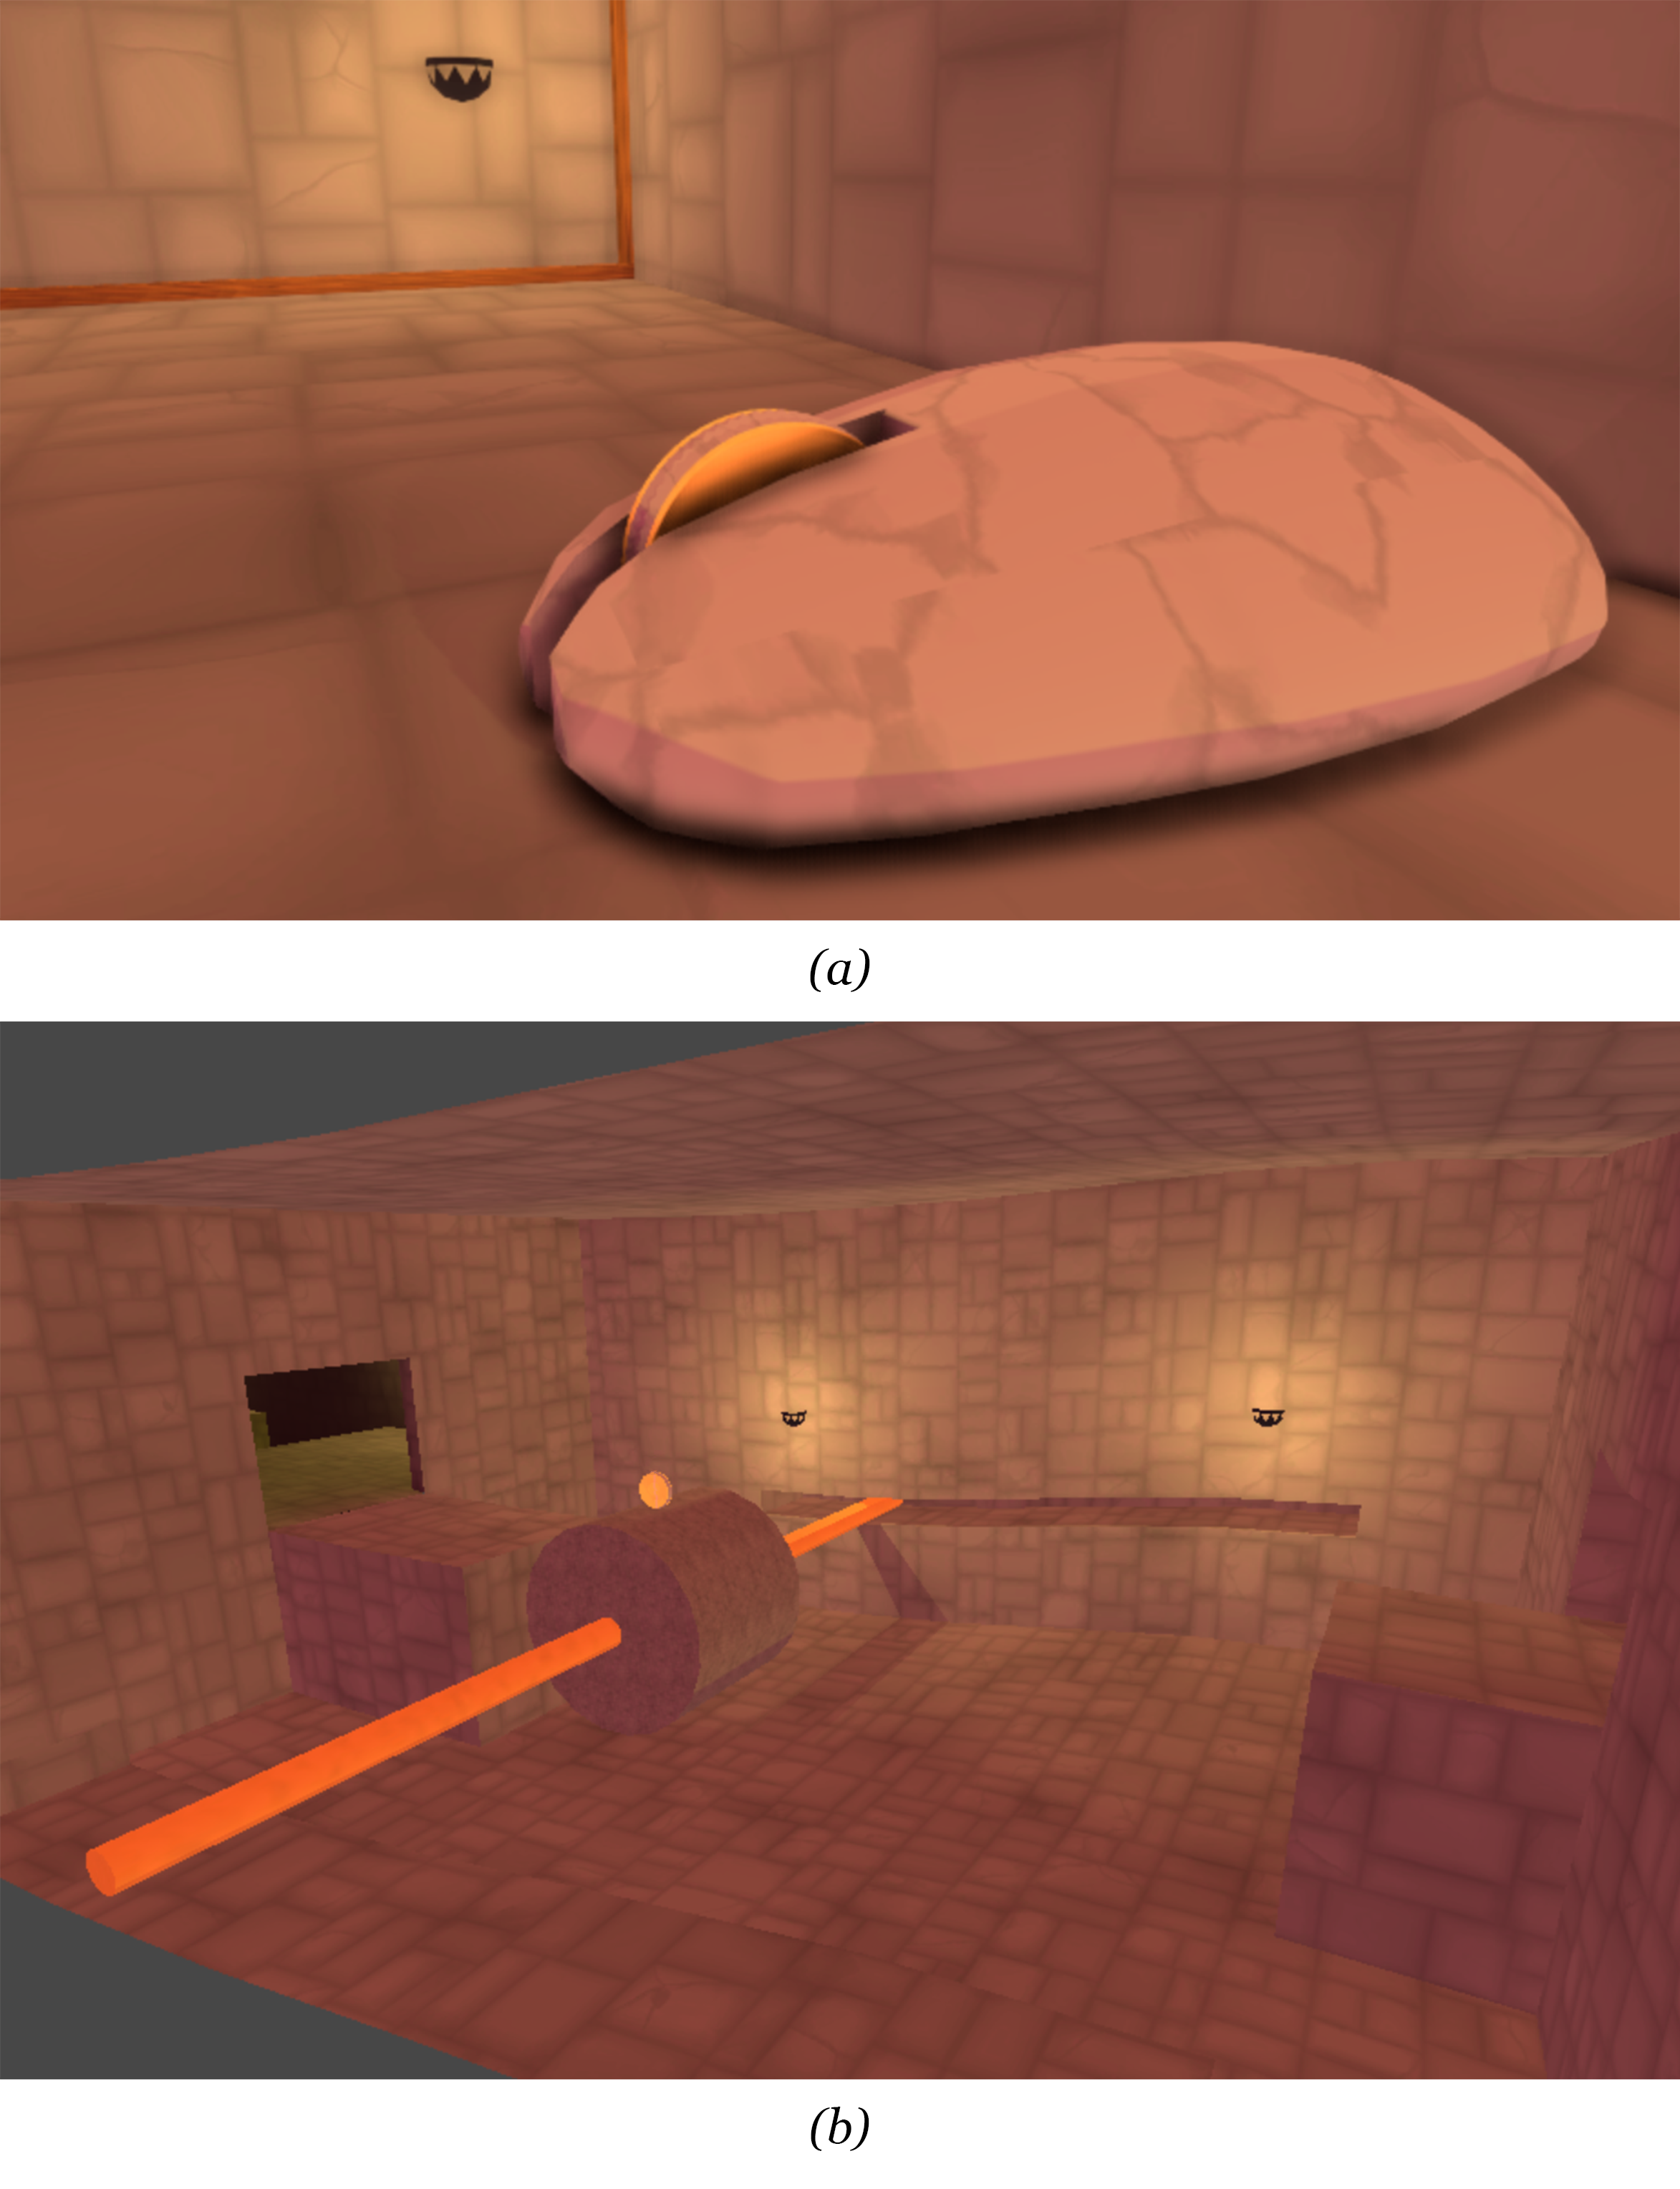
\includegraphics[width=0.6\textwidth]{PrototypeBoth}
  \caption{(a) In-game photo of the prototype as it is presented to a new player (b) The kinaesthetic challenge in focus}
  \label{prototype}
\end{wrapfigure}

Summing up, the described challenge acted as the focal point of the application phases of playtesting and ideation while the method as a whole was the focus of the last evaluation phase with the focus group interview. The next two sections will address the substance of the proposed method and the relevant findings during the two first phases of application and the impressions of the participants from the last evaluation phase. They will be divided into sections representing the context of their use: playtesting and ideation.

\subsection{A Playtest}
The workload of identifying relevant information regarding the six aspects of time, location, direction, modality, dynamics and expression from the framework has been delegated to a playtesting phase in the simplified method. The way this is done is that the interviewer conducting the playtest adhere to a number of questions during the playtest. The questions are divided into two parts: before the identified challenge is attempted and right after. These two phases reflect the phases of pre-action and post-action in the framework and are thereby related to perceivable feedforward and feedback. The questions have been formulated to echo the six aspects in a feedforward setting and a feedback setting and are preluded by a contextual question limiting the scope of the following questions totalling the questions to 14. Each question is, additionally, asked with relevance to both the physical world and the game world, so each question can be said to be two-fold, thereby covering the two dimensions of the framework.

\begin{enumerate}
  \item \textbf{Feedforward}
  \begin{enumerate}
    \item What action would you invoke to overcome the challenge?
    \item When would you apply this action and when would you stop?
    \item Where would you apply this action?
    \item In what direction would you apply this action?
    \item Is there something visually, audibly or tangibly that instructs you how to apply this mechanic?
    \item How much force, speed or acceleration do you think you need to apply?
    \item Do you think you need to apply a certain kind of attitude when applying the action?
  \end{enumerate}
  \item \textbf{Feedback}
  \begin{enumerate}
    \item Now that you have invoked the action, do you feel it was effective in overcoming the challenge?
    \item Did you feel that the action and the effect happened synchronously?
    \item Did you feel that the action and the effect happened at the same location?
    \item Did you feel that the direction of the action was parallel to the direction of the effect?
    \item Did you feel that there was any visual, tactile or audible feature that arose as a consequence of your action?
    \item Did you feel that the amount of force/speed/acceleration from your action was apparent in the effect?
    \item Did you feel that the attitude you applied in your action was apparent in the effect?
  \end{enumerate}
\end{enumerate}

As the questions were formulated they were evaluated by using them in the context they were created for: a playtest. The focus of the playtest was, as discussed earlier, the challenge in the constructed prototype. The way the playtesting was conducted was that I sat down with each participant separately and let them play through the first three minor challenges without instructing them in anything other than letting them know that at a point, I would stop them and ask them some questions. As the playtesting participant reached the challenge in focus I asked them to halt the movement of the playable figure and allowed them to look around in the game world without progressing the challenge. With the game still running, I went through the first seven questions in the given order, waiting for the participant to answer each accordingly. Each question was additionally followed up by a request for elaboration, mostly by asking why they answered what they did. As the participants answered, I wrote down their answers in the form of notes to be used as collected data in the ideation phase. As the final question was discussed I gave back the reins with the encouragement of applying the action they answered the first question with. If the action was successful in overcoming the challenge I carried on with the last seven questions, if not I asked the first seven questions once more, this time with the participant having gained new knowledge.

What was clear from the perspective of the interviewer was that the universal nature of the questions led to some of the questions seeming trivial. As an example, when inquiring about the questions regarding time (1b and 2b), as an interviewer, I was awaiting an affirmative answer, not expecting any other reply, and as a consequence, a feeling of the question as being unconstructive arose. This same consideration was also voiced during the focus group interview. Here, the participants suggested that the playtesting interview should be conducted in a semi-structured way with the questions acting as a starting point, but as the interview goes on the interviewer follows the flow of conversation. This suggestion, in addition to a suggestion of digging even deeper in elaboration on some questions like dynamics and modality (1e, 1f, 2e and 2f), I welcome. What is apparent from the test is that the questions should be considered a checklist to be answered through relevant discussion between the interviewer and the playtester in no particular order other than the first question in each section being asked first.

With that said, this alteration requires diligence of the interviewer since the task of categorising the data becomes more complex, but most importantly keeping on-topic becomes of high importance. It is possible to disregard these two tasks, but let me provide one argument for each task for why they should not: (1) The task of categorisation should not be disregarded because the categorisation inherently provides information on where a weakness or a strength in the design lies and if disregarded can lead to designers focusing on coupling on an aspect that is inappropriate for what the playtester actually experienced. Vice versa, the task of categorisation could be given to the designers, leaving them to code the data \cite{cresswell}. What is inappropriate with this approach is that tacit knowledge from the actual playtesting situation is lost \cite{cresswell}.

Conclusively, I suggest that the categorisation task should be prioritised and should be conducted by the interviewer as close in time to the playtesting as possible. (2) The task of keeping on-topic should not be disregarded because the scope of the method is relatively narrow. What can happen if the subject matter is deprioritised is that the playtesting session can evolve into a general playtesting session with discussions concerning graphical glitches, similarities to other games, aesthetic qualities, etc. which can end up being irrelevant for the purpose of the playtest, which is to gather data on the intuitiveness of a kinaesthetic challenge.

One other interesting finding was the difficulty of the participants to express and identify what they felt and why they felt the way they did. This lead to interesting replies such as when asked how much force, speed or acceleration they thought they would need to apply in the context of scrolling the mouse wheel fast enough to use the barrel as a ramp for the playable figure, the participant answered that he thought he would need as much force as one would apply to get to the bottom of a webpage. This can be explained by the fact that the method, as well as the framework, is highly concerned with knowledge residing in the lebenswelt \cite{dourish}: the intersubjective unconscious knowledge and understandings gained from experience. This knowledge is tacit knowledge in the way that it is hard to explain to another person. What makes this example so important is that intersubjectivity is used to answer the question in a way that many would understand because most have experienced the situation of wanting to scroll to the bottom of a page: It is forceful and fast. From this finding, I suggest that any utilisation of the proposed method include an explanation from the interviewer in the playtesting processes of the possibility of using past experiences as examples to identify what is felt and how it is felt.

\subsection{An Ideation}
After data has been collected, the task of plotting the data into a model to get a visual representation of what is perceived is undertaken in the ideation process of a development team or, in a bigger studio, the design team. The model for the proposed method has been considerably simplified relative to the framework. The most noteworthy simplification has been the collapse of the dimensions of feedforward and feedback. This was done as a consequence of wanting to adapt the framework into a nimble straightforward method that is accessible enough to use, that it can be a tool in a practical setting. This was done because I wanted to adapt the framework into a method for sketching \cite{buxton}. Why that had to cost the distinction between feedforward and feedback is grounded in what was earned from the distinction. In the framework, the distinction makes it clear whether or not a challenge is feedforward or feedback heavy, the analytical gain of this should be obvious and the notion that \citeA{frogger} themselves made distinctions mainly for the purpose of analysis \cite[p. 5]{vermeulen} reassures my decision, because, as a tool for sketching, the purpose of sketching is not for the sake of analysis but to spark ideas and open up a design: ``Their value lies not in the artifact of the sketch itself but in its ability to provide a catalyst to the desired and appropriate behaviors, conversations, and interactions'' \cite[p. 113]{buxton}.

Additionally, being able to look at a design challenge holistically can create better products \cite{buxton}, and this is counteracted if the designers were to make an incision at a point in the challenge and say from this point feedforward and feedback relates. With this said, there is value lost in the collapse. A value that is also relevant for a design team, and I leave it up to future interpretations to find a way to feed this value from the framework into the method. Perhaps a last analytical phase could be beneficial to a design team.

All other changes have been made to ease the drawing of a model to be used in the method, most importantly reducing the complexity of shapes. This decision should not be brushed off as just being a whimsical side note. When pen and paper sketching is such a wide-used method of sketching in a world with increasing technological gadgets promising to enhance the sketching experience, it is because grabbing a pen and a piece of paper is accessible. No app is needed, no processing power is required other than one's own brain. This is why I have put effort into reducing the framework into three lines: they are fast to draw and do not require accurate brush strokes, meaning that they can hopefully be drawn over and over in the same sketching session without becoming a nuisance. The model can be seen in figure \ref{fart}. Because of the model's resemblance to a bending river I have chosen to name the method \textit{the Four-Angled River Technique} (FART) for purposes of simple reference. From the top left in a clockwise order, the letters represent inherent information, functional information, augmented information, ludic action and action.

\begin{wrapfigure}{i}{0.5\textwidth}
  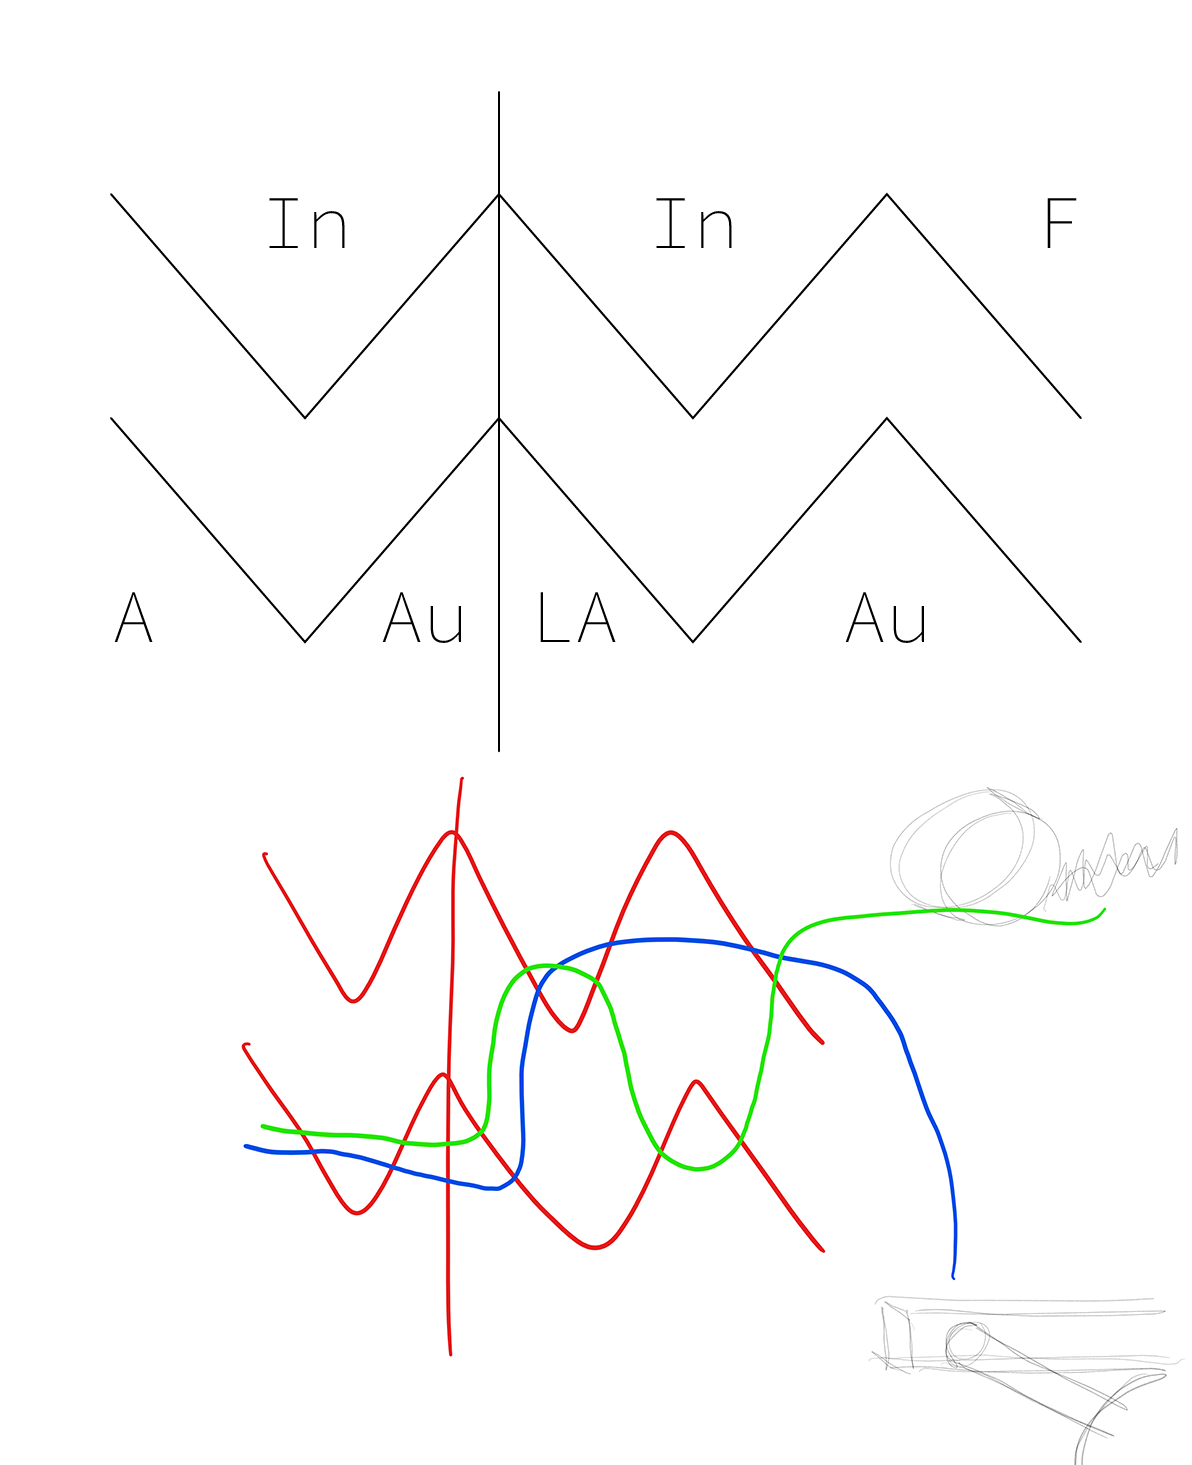
\includegraphics[width=0.5\textwidth]{FARTBoth}
  \caption{The Four-Angled River Technique. Above is the formal form and below is how it could look in practice}
  \label{fart}
\end{wrapfigure}

Before presenting the method to the participants I conducted a short lesson in the meaning of inherent, augmented and functional information. During the lesson I mirrored the notion of \citeA{frogger} in saying that inherent information is preferred over augmented information because of the lesser effort needed for psychomotor tasks compared to cognitive tasks, which means a task requires less attention, thereby allowing for internalising the controls \cite{calleja}. While promoting inherent information, a point was also made that should an inherent solution be too costly, augmented information is still preferred over no coupling, and may, in some situations, be more appropriate.

After the lesson, I presented them to the method and drew the model (see figure \ref{fart}) on an adjacent whiteboard. I then provided them with the data I had gathered from the playtests and presented them with a task: With the data and their own impressions, they should come up with ideas to improve the design of the kinaesthetic challenge from my prototype using the method. In effect, they were to role-play as a design team tasked with improving a design.

What I noted when observing the participants was that an initial confusion of how the couplings were to be visually represented was slowly replaced by a more fluid workflow of discussion and drawing. One thing that stood out, was that no lines were connected to functional information and no couplings were made between augmented and inherent information. From this I draw two conclusions: (1) The identification of functional information becomes implicit in the context of focusing on conveying meaning of how to overcome a challenge. In a sense, all ideas with the intent of making the general purpose clear to the user can be labelled as ideas providing functional information \cite{frogger}. Therefore, starting a coupling from the visual representation of functional information can seem redundant, when in fact it is not. A coupling is made between action and meaning through inherent information and augmented information. This leads me to the second conclusion: (2) The lesson was insufficient in teaching the proper skills needed to take full advantage of the method. First, the lesson should have provided the information discussed in the first conclusion and the addition that couplings are made between action or ludic action and functional information through augmented and inherent information, not between individual information types. This way of thinking of a coupling as a stream of information travelling through delineating channels may be beneficial for the understanding of the value of the method. Secondly, the lesson, as it was, focused on augmented information, inherent information and how they are distinct from each other. It should have also provided information on, not just that it can, but \textbf{how} a coupling can travel through both types of information, as was the case in the analysed example from \textit{The Legend of Zelda: Skyward Sword} where the affordance between the sword and the Deku Baba provided a coupling that travelled through augmented information and inherent information. Finally, the lesson should have provided an exemplary demonstration of how the method could be used with a dissimilar challenge to show the participants how the method is intended to be used, but with emphasis on the possibility of interpretation.

In the focus group interview that followed, granularity was a meaningful topic. One participant voiced the opinion that he would have preferred a way to label the couplings according to what the information was regarding in order to better compare different ideas. Other participants counterargued that this was against the purpose of a sketching tool, echoing the notion from \citeA{buxton}, as discussed earlier, with the sketch as an artefact having no value other than the inspirational value it provided in the creation of it. Agreeing with the majority of the participants, there still lies some truth in the one's suggestion since being able to discern the existing couplings would perhaps elevate the conversation by having recognisable couplings to relate to while sketching new ones. Again, I leave it up to future interpretations to explore the possibility of including a way of labelling information, however, using the words of \citeA{buxton}, when the pen reaches the end of a line representing a coupling, ``if you can’t afford to throw it away when done, it is probably not a sketch'' \cite[p. 111]{buxton}. Other than the point of labelling, the participants considered the method as sufficient in its granularity and expressed that the level of detail should be kept to the current minimum for the method to be constructive in an ideation process.
